\documentclass[t, xcolor={dvipsnames}]{beamer}

\usepackage{tipa}
\usepackage{eso-pic}
\usepackage{graphicx}
\usepackage{svg}
\usepackage{listings}
\usepackage{wrapfig}
\usepackage{scrextend}
\usepackage{subfig}

\setsvg{svgpath = img/}

\makeatletter
  \newenvironment{withoutheadline}{%
    \setbeamertemplate{headline}[default]
    \def\beamer@entrycode{\vspace*{-\headheight}}
    \setbeamertemplate{footline}[default]
  }{}
\makeatother

\usetheme{Malmoe}
\usecolortheme{dolphin}
\setbeamercolor{structure}{bg=red}

\title{\vspace{0.8cm}Automatic Birdsong Recognition}
\author{Victor F. L. Rodrigues}
\institute{School of Computer Science\\ The University of Manchester}
\titlegraphic{\includesvg[height=15mm]{UniOfManchesterLogo}}
\logo{\includesvg[height=10mm]{UniOfManchesterLogo}}

\begin{document}

%\usebackgroundtemplate{%
%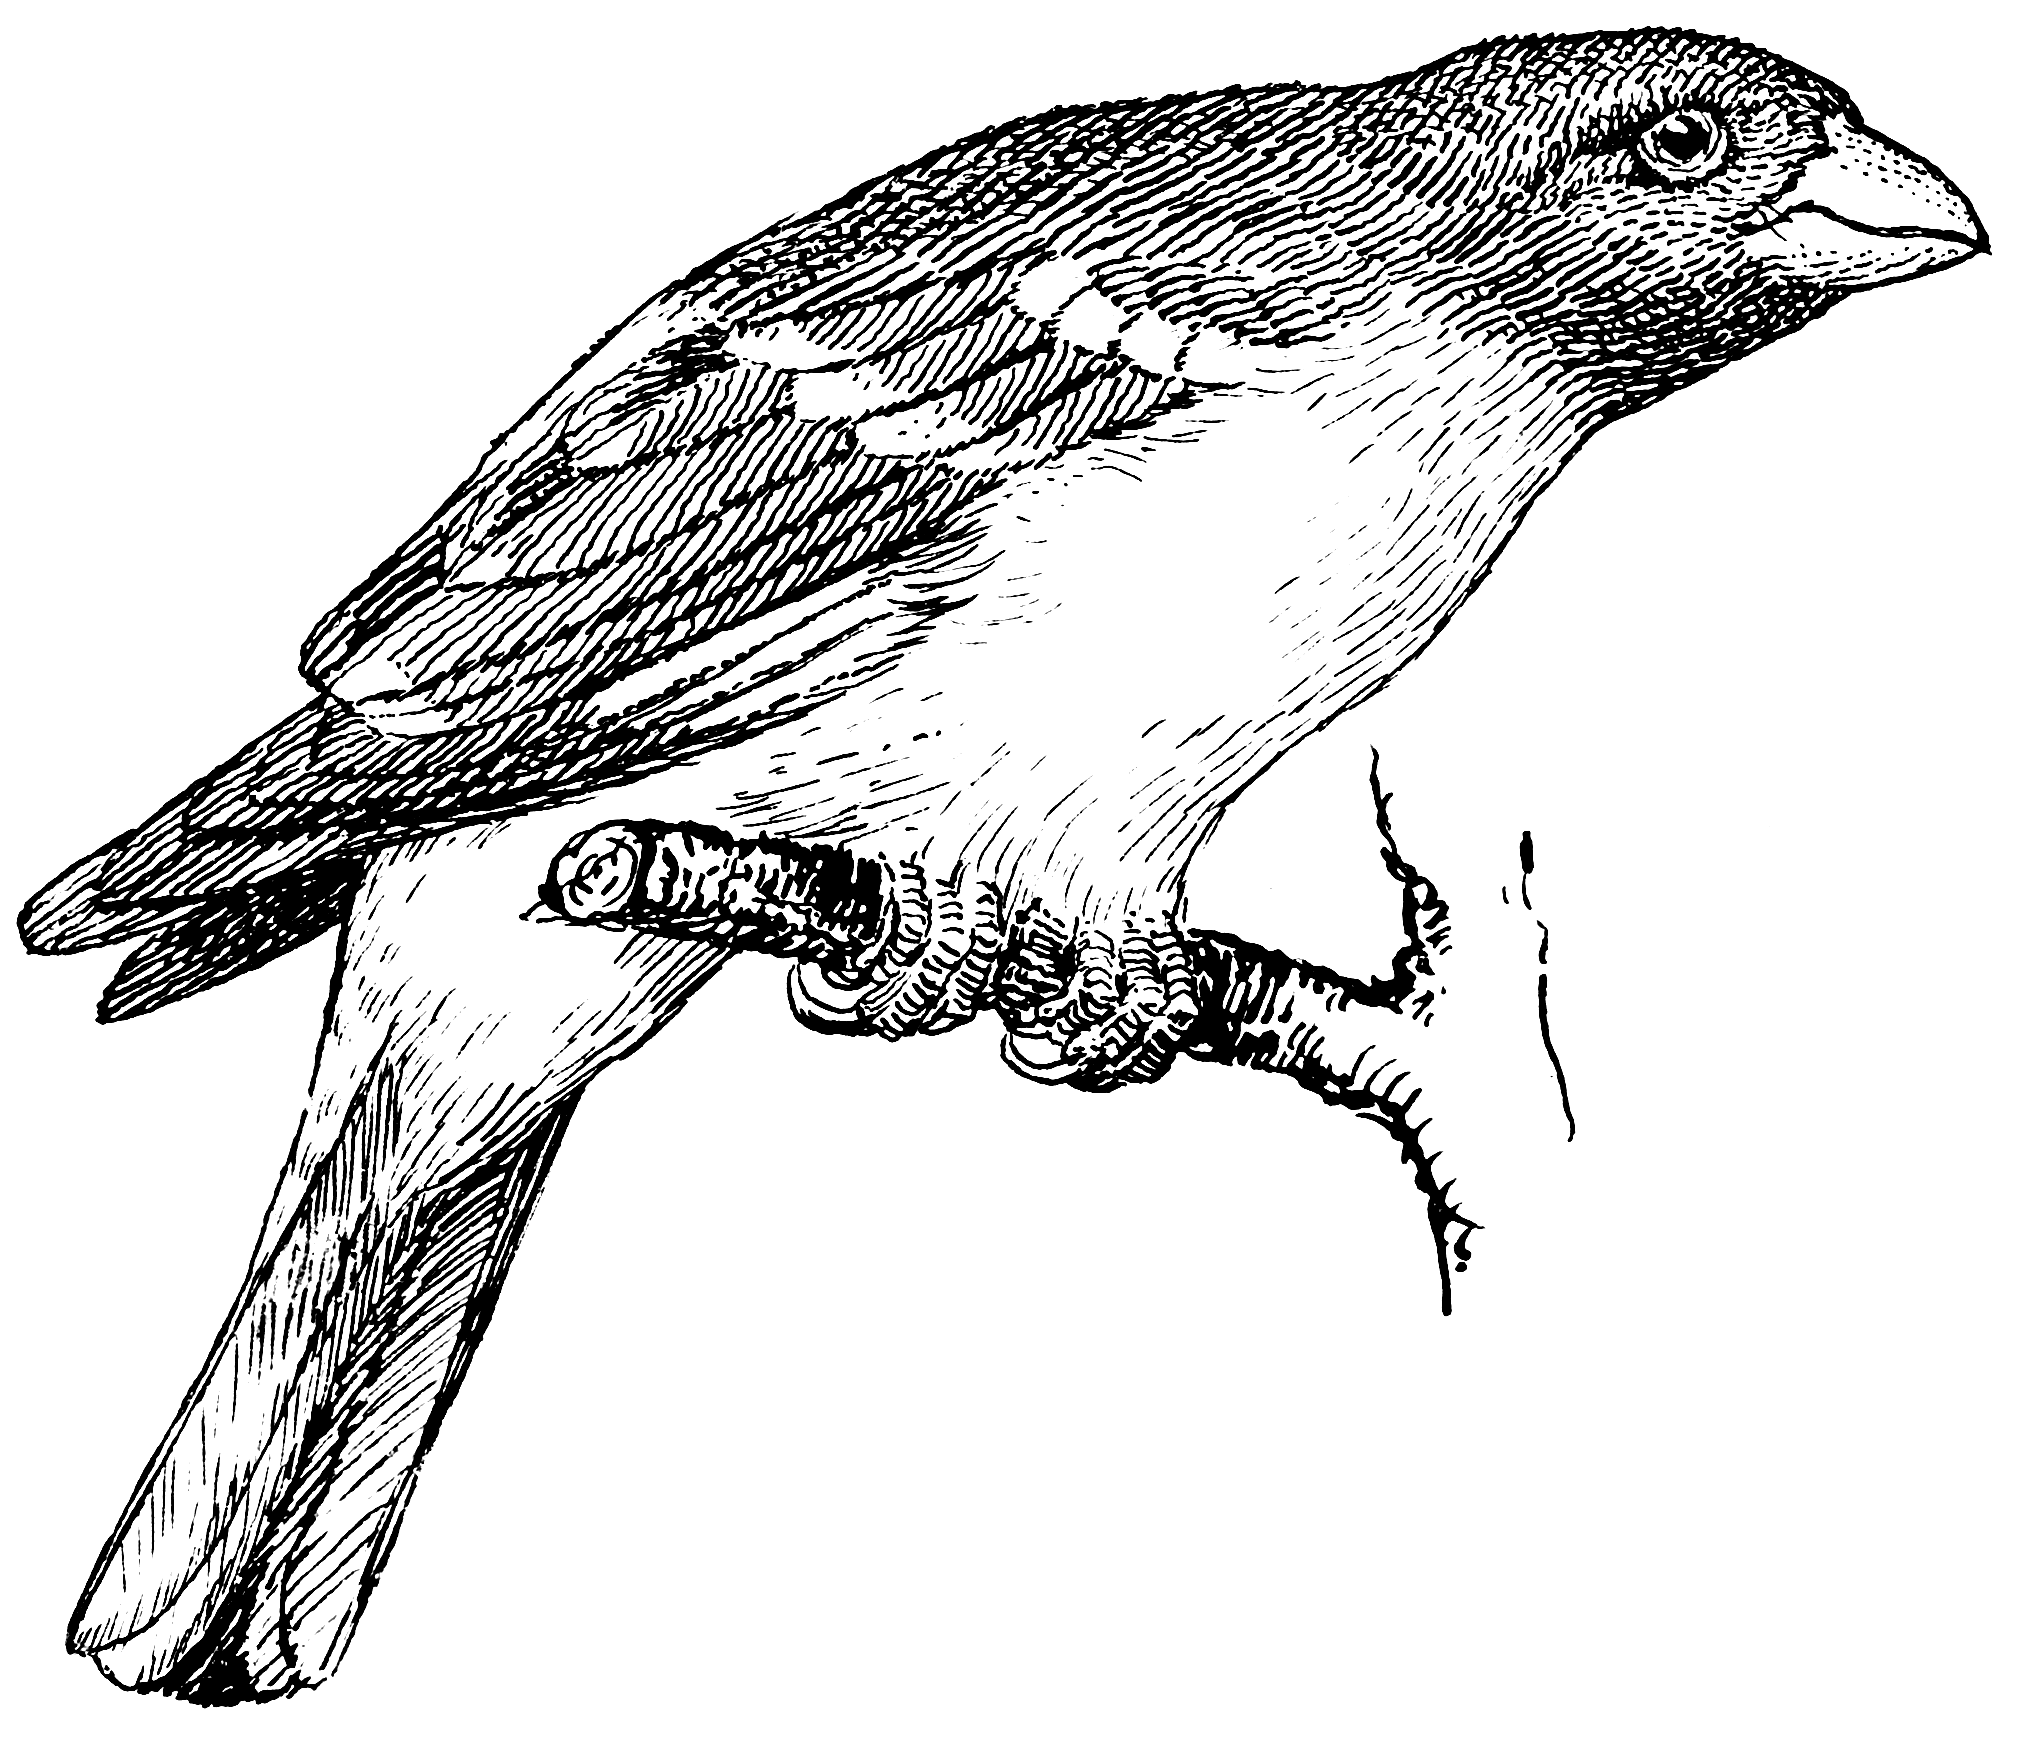
\includegraphics[width=0.5\paperwidth,height=0.5\paperheight,keepaspectratio=true]{img/Grossbeak_(PSF).png}
%}

\begin{withoutheadline}
  \begin{frame}[plain]
    \begin{wrapfigure}{L}[20cm]{0.23\textwidth}
      \vspace{0.2cm}
  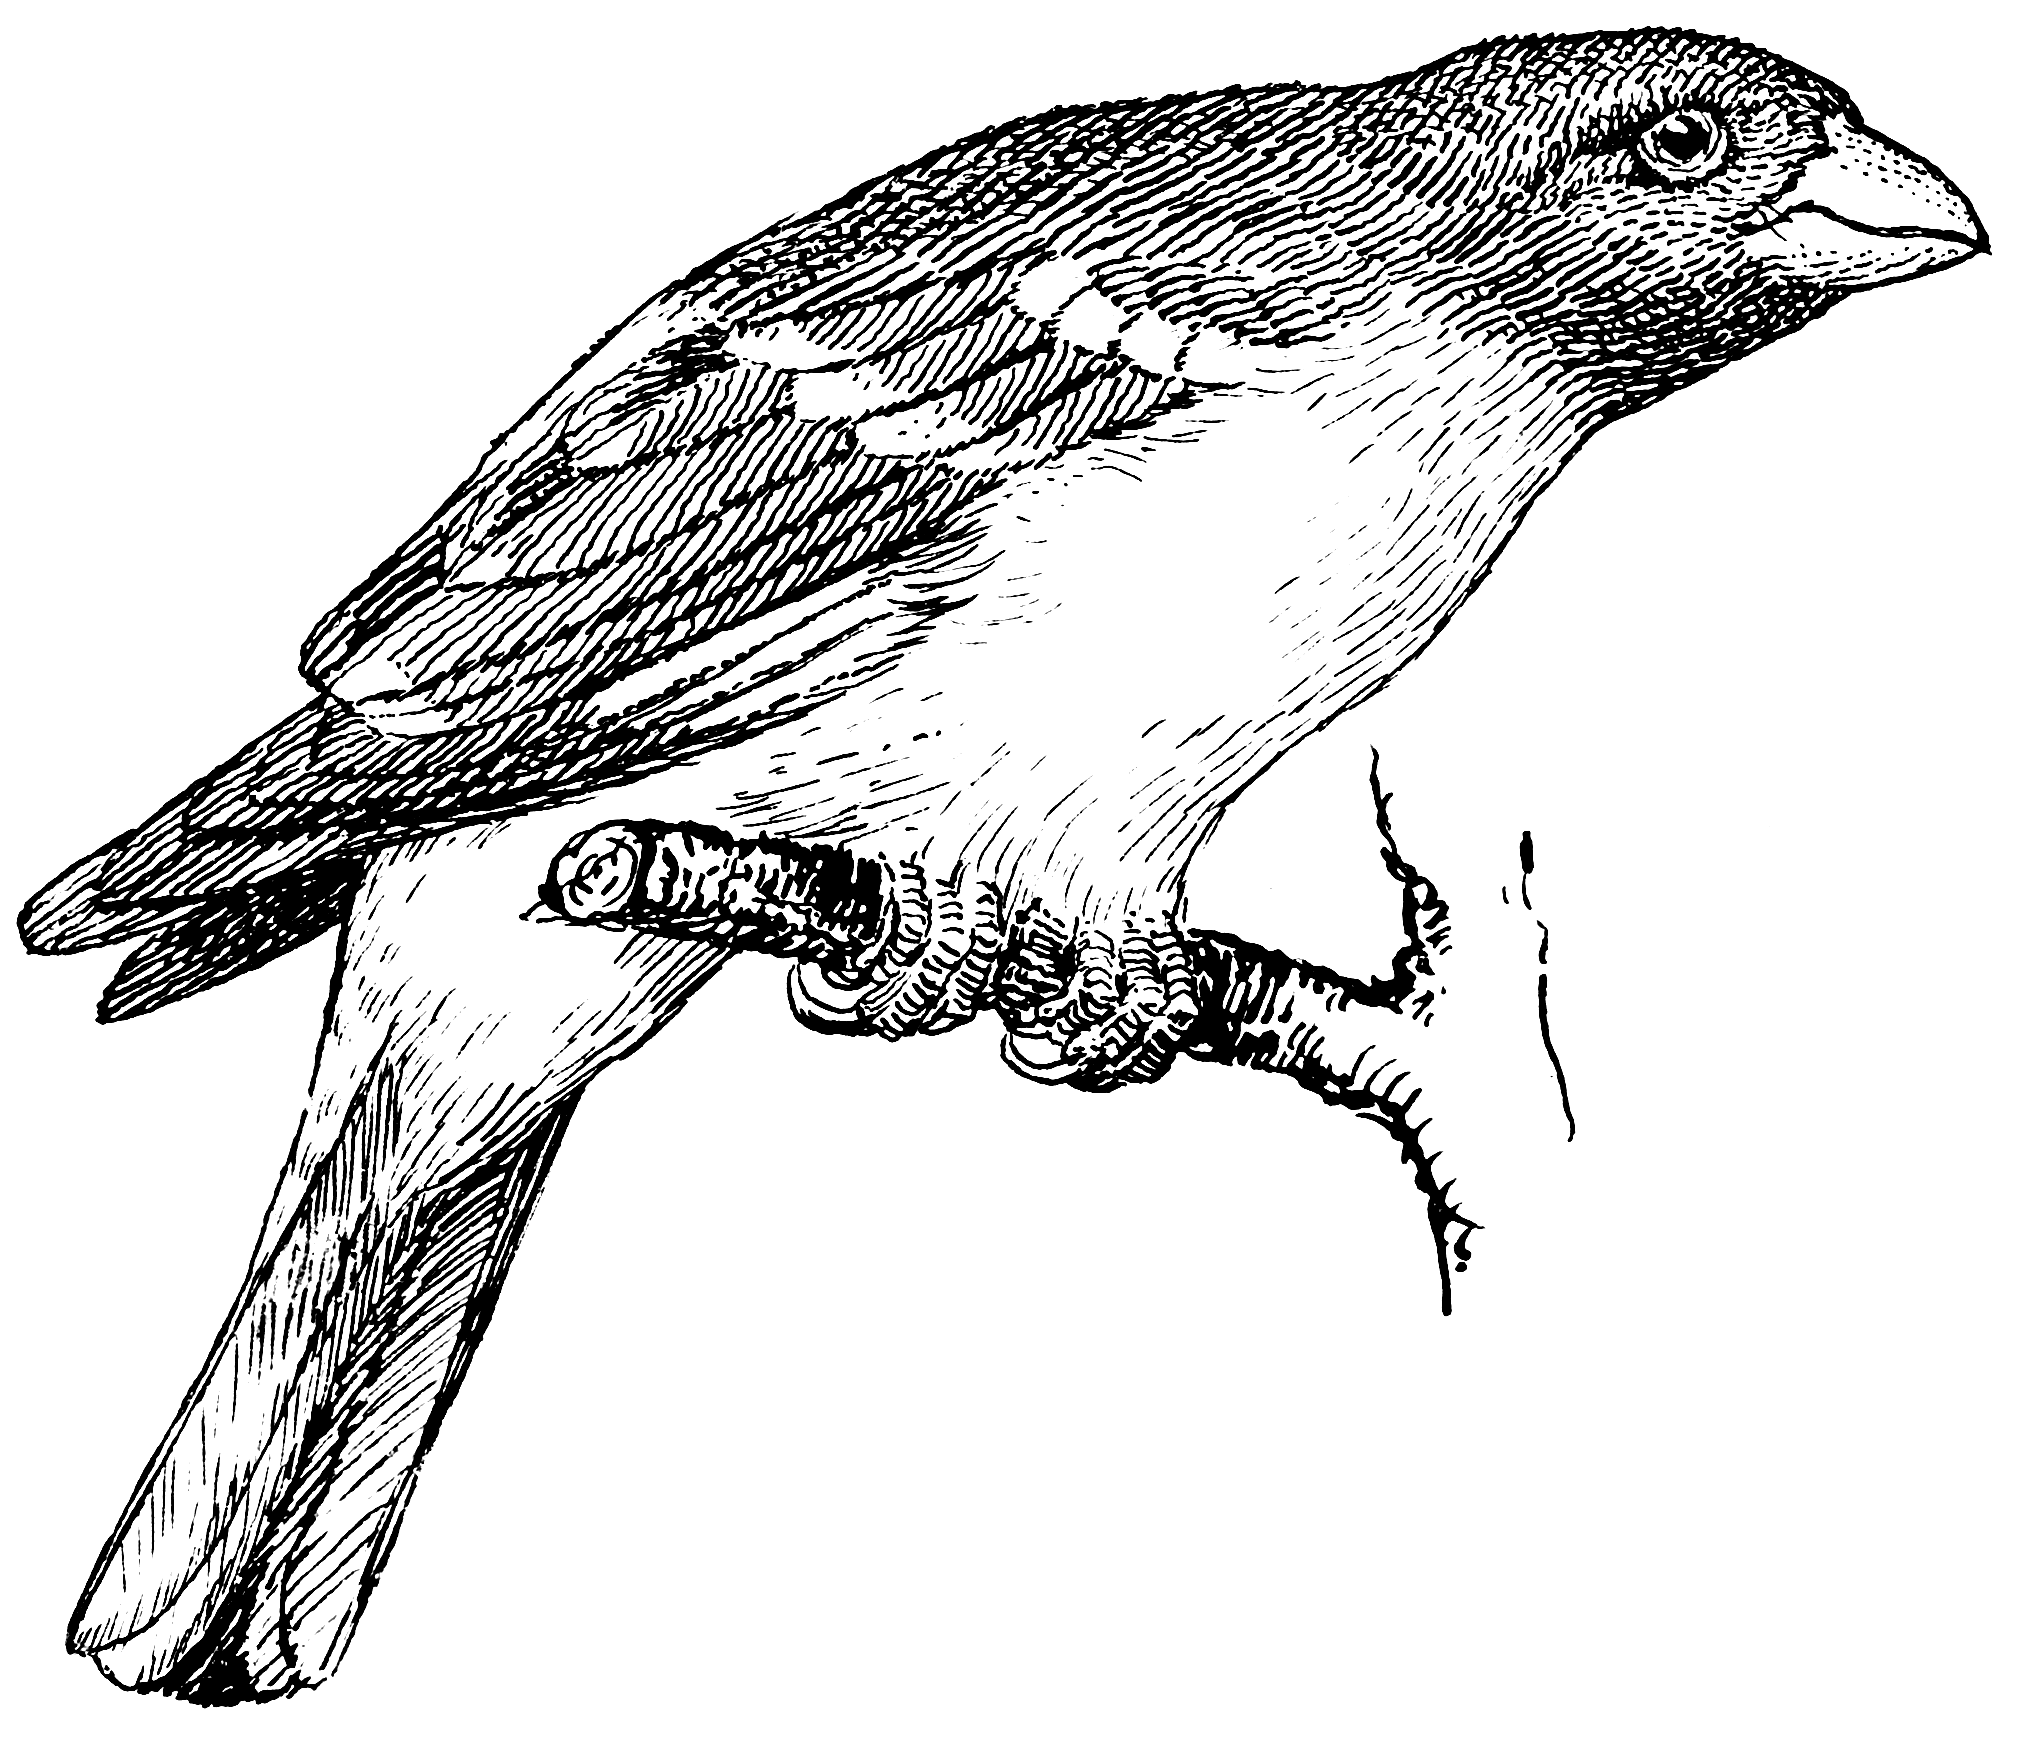
\includegraphics[width=0.5\paperwidth,height=0.5\paperheight,keepaspectratio=true]{img/Grossbeak_(PSF).png}
    \end{wrapfigure}
    \titlepage
  \end{frame}
\end{withoutheadline}

\usebackgroundtemplate{}

%-------------------------------------------------------------------------------

\section{Bird-Song Recognition}
\subsection{In Birdwatching}

\begin{frame}[fragile]
  \vspace{0.5cm}
  {\bfseries\Large How birdwatchers do it}\\
  \vspace{0.5cm}
  \begin{addmargin}{0.5cm}
    \begin{itemize}
      \item Listen to frequency sweeps, tones, repetitions
      \item Spectrographic analysis\ldots
    \end{itemize}
    [show clean specgram?]
  \end{addmargin}
\end{frame}

%-------------------------------------------------------------------------------

\subsection{As a classification problem}

\begin{frame}[fragile]
  \vspace{0.5cm}
  {\bfseries\Large How birdwatchers do it}\\
  \vspace{0.5cm}
  \begin{addmargin}{0.5cm}
    \begin{itemize}
      \item Listen to frequency sweeps, tones, repetitions
      \item Spectrographic analysis\ldots
    \end{itemize}
  \end{addmargin}
  \vspace{0.5cm}
  {\bfseries\Large How a computer might do it}\\
  \vspace{0.5cm}
  \begin{addmargin}{0.5cm}
    \begin{itemize}
      \item Similar problems exist: Vocal recognition, music identification, whalesong classification\ldots
      \item A multi-class/multi-label classification problem
      \item Features are extracted from spectrographic analysis
      \item Machine learning is used to classify the data
    \end{itemize}
  \end{addmargin}
\end{frame}

%-------------------------------------------------------------------------------

\section{Processing}

\begin{frame}[fragile]
  \vspace{0.5cm}
  {\bfseries\Large The data}
  \vspace{0.5cm}
  \begin{addmargin}{0.5cm}
    [show waveform]
  \end{addmargin}
\end{frame}

\begin{frame}[fragile]
  \vspace{0.5cm}
  {\bfseries\Large The data}
  \vspace{0.5cm}
  \begin{addmargin}{0.5cm}
    [show waveform]
    [show specgram]
  \end{addmargin}
\end{frame}

% In these frames talk about visible shapes and sweeps. maybe we could extract
% information or statistics on the frequency disitrbutions and the audiable
% repetitions? But maybe we have too much noise... leads to next section

%-------------------------------------------------------------------------------

\subsection{Noise Reduction}

\begin{frame}[fragile]
  \vspace{0.5cm}
  {\bfseries\Large Too much noise!}\\
  \vspace{0.5cm}
  \begin{addmargin}{0.5cm}
    \begin{itemize}
      \item Signal to noise ratio might interfere with our extraction
      \item An \emph{automatic} noise reduction method is requried.
      \item Standard computer vision techniques can be used:
      \begin{itemize}
        \item Median filtering
        \item Thesholding
        \item dilation \& erosion\ldots
      \end{itemize}
    % after a few parameter tweaks we get something more like this...  
    \end{itemize}
  \end{addmargin}
\end{frame}

% Too much noise to run edge detector. Some background noise is not part of the
% signal we are interested in. we want to minimise the SNR.
%
% Automatic noise reduction is necessary to increase the number of samples we
% can use. This is tricky, as noise reduction parameters are not global. We may
% need to automatically fit params to each recording, or make do with a general
% setting, which might be difficult to find.
%
% A combination of computer vision algos can be used

%-------------------------------------------------------------------------------

\begin{frame}[fragile]
  \begin{figure}[!tfp]
    \centering
    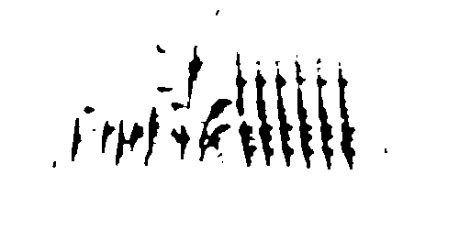
\includegraphics[width=0.8\textwidth]{img/specgram-long-clean}
  \end{figure}

  \vspace{-1cm}

  \begin{addmargin}{0.5cm}
    \begin{itemize}
      \item Imperfect results might be close enough through statistical average
      \item Per-recording parameter fitting would be ideal, but more complex
    \end{itemize}
  \end{addmargin}
\end{frame}

% Point out imperfect cleanup. Note that this is impossible w/ global
% parameters, but maybe it doesn't have to be perfect in the first place given
% the quantity of samples that we will have.

%-------------------------------------------------------------------------------

\subsection{Feature Engineering}
\begin{frame}[fragile]
  \vspace{0.5cm}
  {\bfseries\Large What really matters?}\\
  \vspace{0.5cm}
  \begin{addmargin}{0.5cm}
    [show clean specgram from before]
    \begin{itemize}
      \item Dominant frequency domains per species (pitch)
      \item Characteristic patterns, we can see structure
      \item Discreet groupings, repetitions, and syllables can be identified
    \end{itemize}
  \end{addmargin}
\end{frame}

%-------------------------------------------------------------------------------

\begin{frame}[fragile]
  \vspace{0.5cm}
  \begin{addmargin}{0.5cm}
    \begin{itemize}
      \item Another approach: image recognition
      \item Components can be cross-correlated against specgrams
      \item A common approach is template matching:
%      \begin{itemize} \item Find contours and crop section from original
        %      spectrogram \item Apply gaussian blur to improve generalisation
        %      (dimensionality reduction) \item Use result as a template through
        %      cross-correlation mapping against target spectrogram
      %\end{itemize}
    \end{itemize}


%    [show crop of specgram with contours] [show bounding box on original
    %    specgram] [show cross correlation map against specgram] [show
    %    thresholded version]
  \end{addmargin}

    \begin{figure}[!tbp]
      \centering
      \begin{minipage}[c]{0.3\textwidth}
        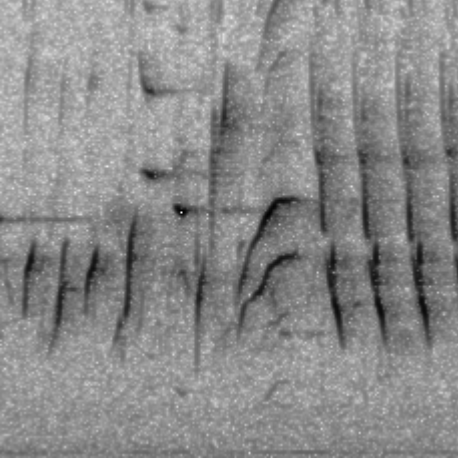
\includegraphics[width=\textwidth]{img/specgram}
      \end{minipage}
      \hfill
      \begin{minipage}[c]{0.3\textwidth}
        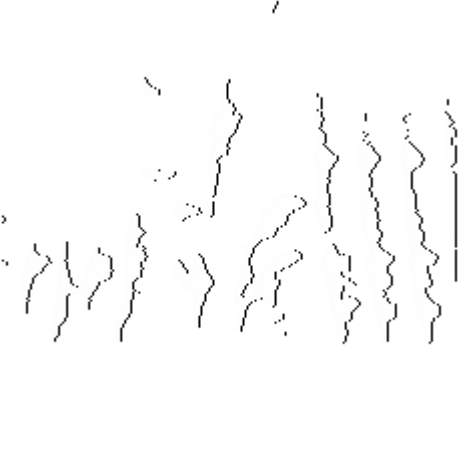
\includegraphics[width=\textwidth]{img/contours}
      \end{minipage}
      \hfill
      \begin{minipage}[c]{0.3\textwidth}
        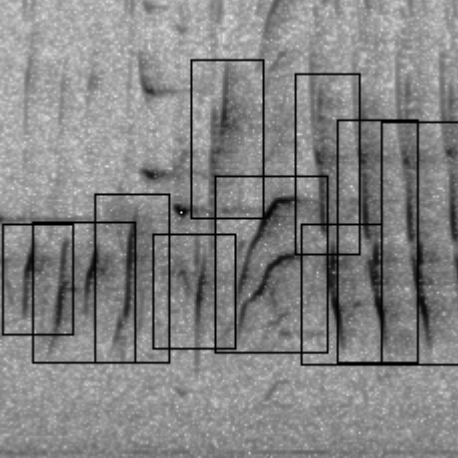
\includegraphics[width=\textwidth]{img/detected-features}
      \end{minipage}
%      \begin{minipage}[c]{0.1\textwidth}
      %      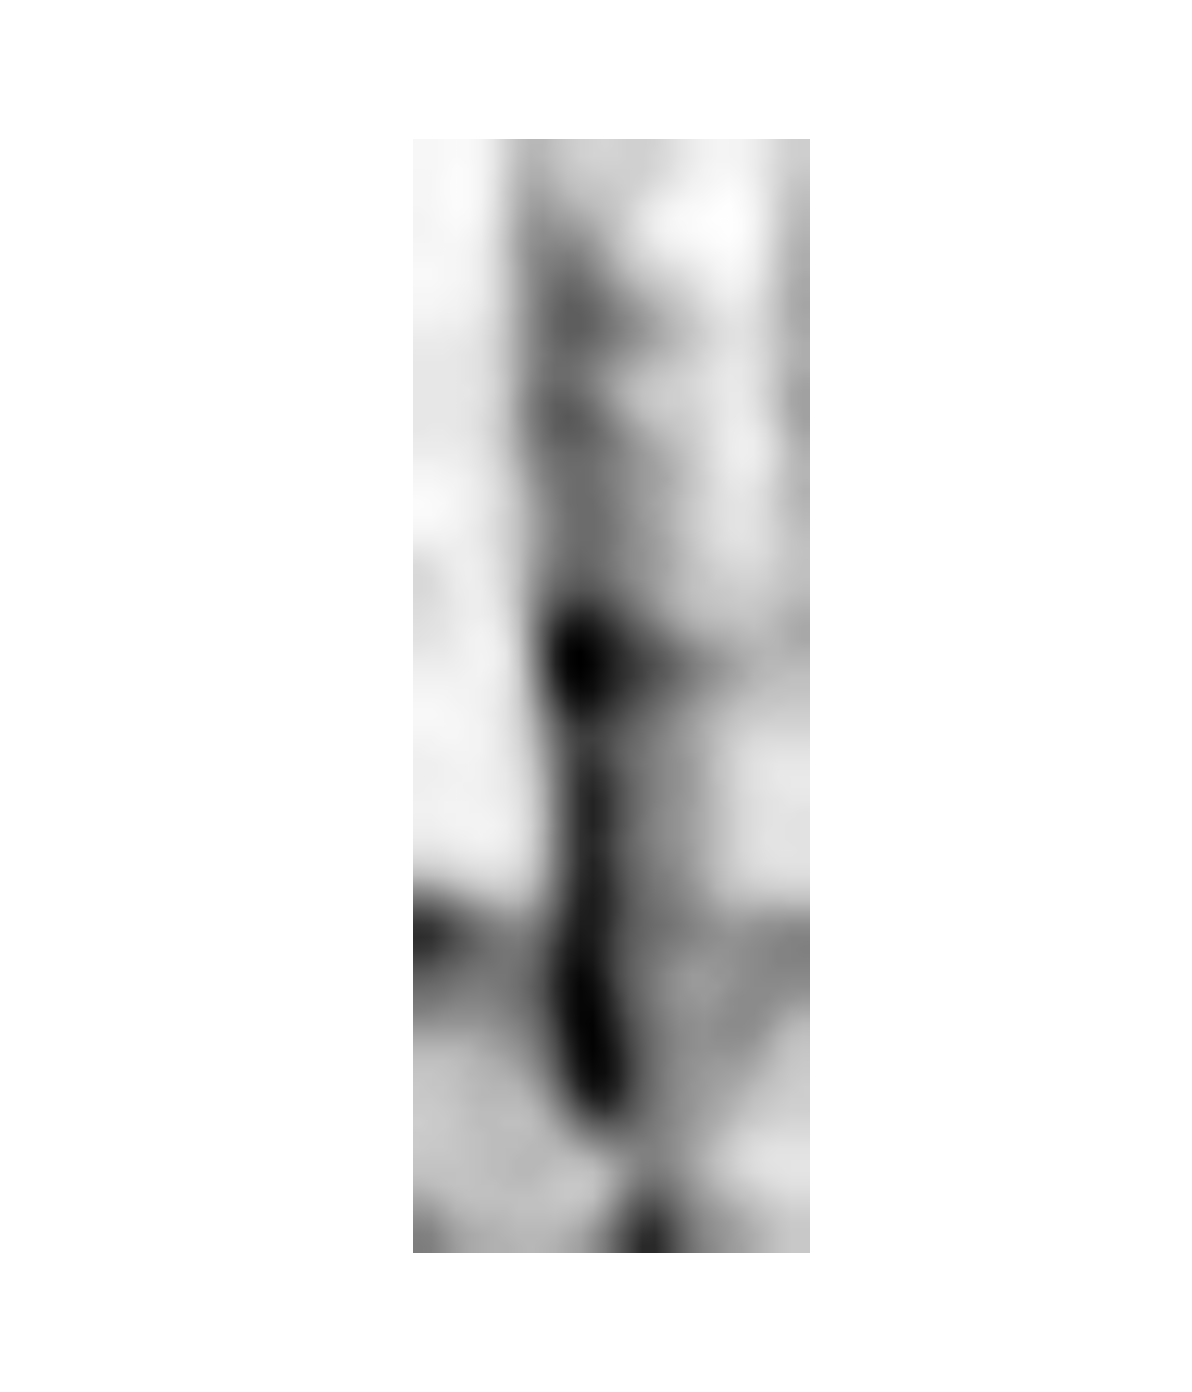
\includegraphics[width=\textwidth]{img/selected-feature}
      %      \end{minipage}% \begin{minipage}[c]{0.3\textwidth}
      %      \includegraphics[width=\textwidth]{img/CCM}
%      \end{minipage}
%      \begin{minipage}[b]{0.1\textwidth}
      %      \includegraphics[width=\textwidth]{img/thresholded-CCM}
      %      \end{minipage}
    \end{figure}
\end{frame}

\begin{frame}[fragile]
  \vspace{0.5cm}
  \begin{addmargin}{0.5cm}
    \begin{itemize}
      \item Another approach: image recognition
      \item Components can be cross-correlated against specgrams
      \item A common approach is template matching:
%      \begin{itemize} \item Find contours and crop section from original
        %      spectrogram \item Apply gaussian blur to improve generalisation
        %      (dimensionality reduction) \item Use result as a template through
        %      cross-correlation mapping against target spectrogram
      %\end{itemize}
    \end{itemize}


%    [show crop of specgram with contours] [show bounding box on original
    %    specgram] [show cross correlation map against specgram] [show
    %    thresholded version]
  \end{addmargin}

    \begin{figure}[!tbp]
      \centering
%      \begin{minipage}[c]{0.3\textwidth}
      %      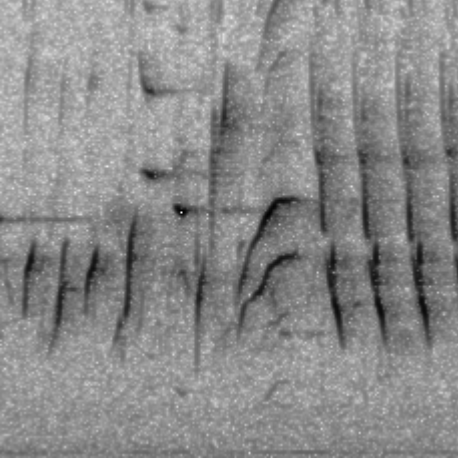
\includegraphics[width=\textwidth]{img/specgram} \end{minipage}%
      %      \begin{minipage}[c]{0.3\textwidth}
      %      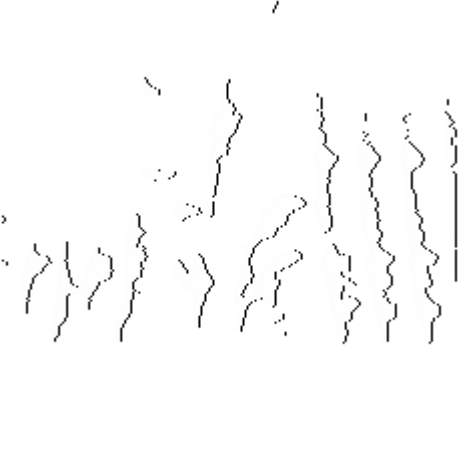
\includegraphics[width=\textwidth]{img/contours} \end{minipage}%
      %      \begin{minipage}[c]{0.3\textwidth}
      %      \includegraphics[width=\textwidth]{img/extracted-features}
%      \end{minipage}%
      \begin{minipage}[c]{0.3\textwidth}
        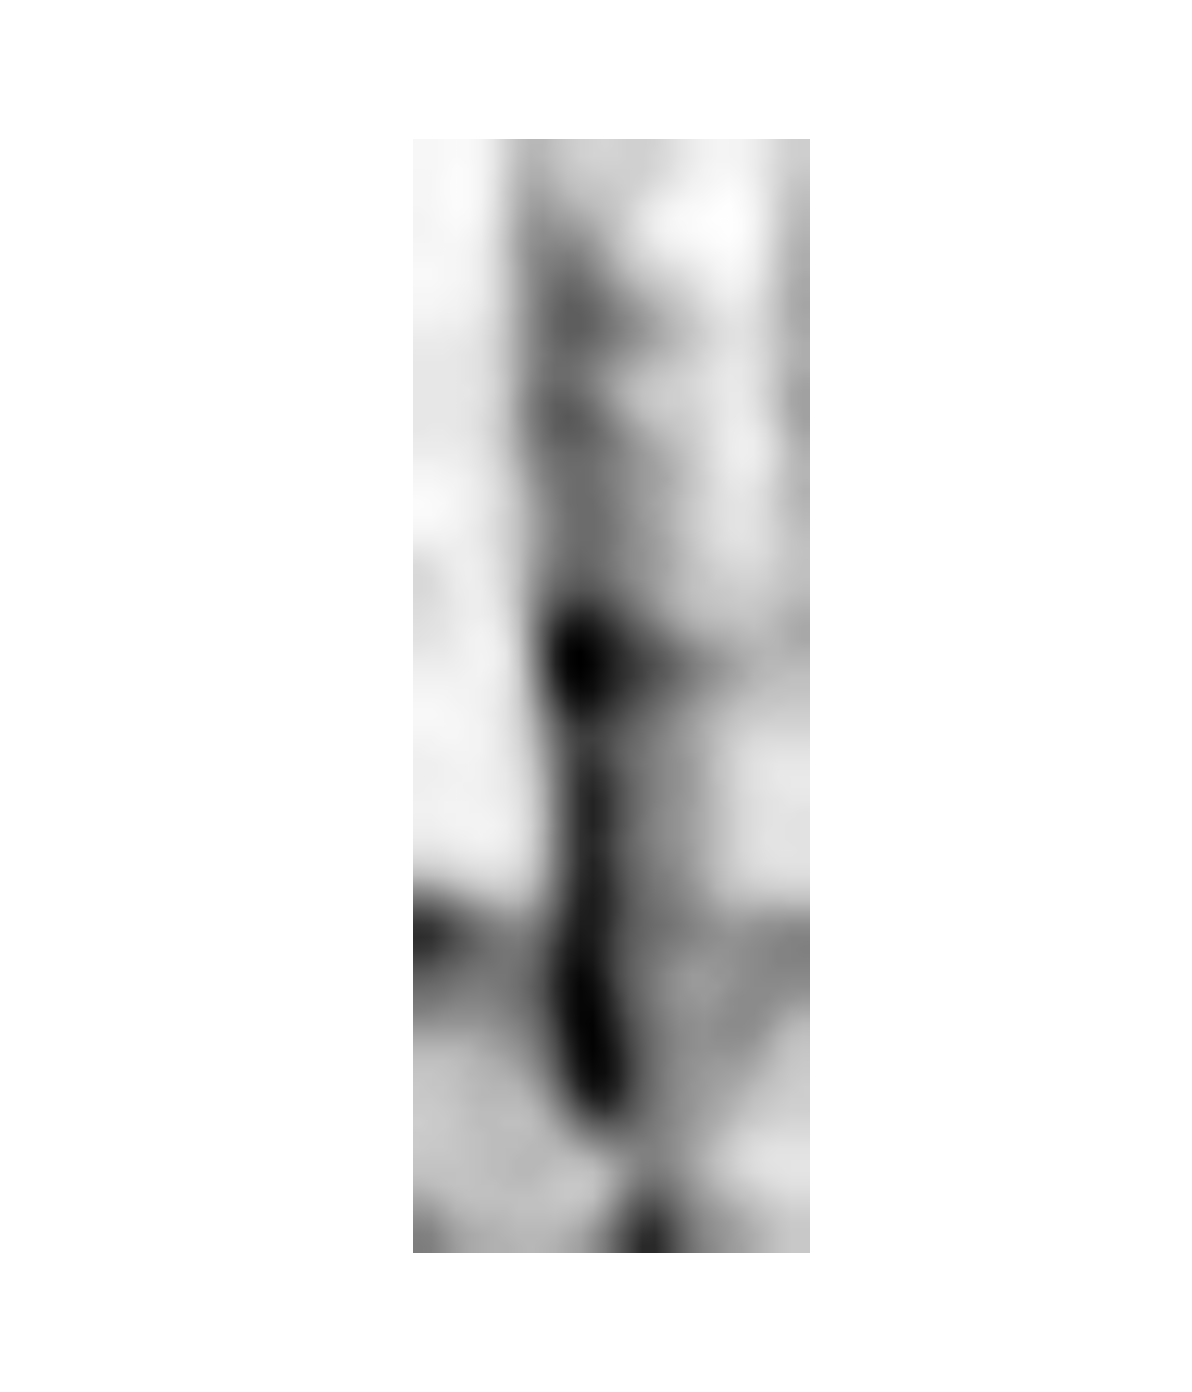
\includegraphics[width=\textwidth]{img/selected-feature}
      \end{minipage}
      \hfill
      \begin{minipage}[c]{0.3\textwidth}
        \fbox{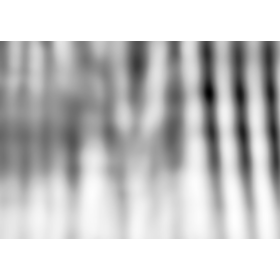
\includegraphics[width=\textwidth]{img/ccm}}
      \end{minipage}
      \hfill
      \begin{minipage}[c]{0.3\textwidth}
        \fbox{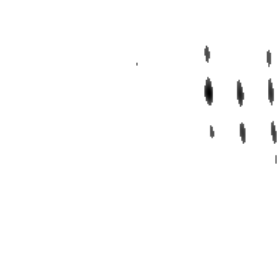
\includegraphics[width=\textwidth]{img/threshold-ccm}}
      \end{minipage}
    \end{figure}
\end{frame}


%-------------------------------------------------------------------------------

\section{Classification}
\begin{frame}[fragile]
  \vspace{0.5cm}
  {\bfseries\Large Classifying the data}\\
  \vspace{0.5cm}
  \begin{addmargin}{0.5cm}
    \begin{itemize}
      \item Decision trees. Random forest, 50 - 500 trees.
      \item One RF per class.
      \item Use all features..
      \item Work with limited set of classes first...
    \end{itemize}
  \end{addmargin}
\end{frame}

\section{}
\begin{frame}[fragile]
  \vspace{0.5cm}
  {\bfseries\Large Conclusion}\\
  \vspace{0.5cm}
  \begin{addmargin}{0.5cm}
    \item Non-trivial classification task..
    \item Possible issues with data sanitation..
    \item Large variation in birdsong between species
    \item not all hope is lost..
  \end{addmargin}
\end{frame}


%-------------------------------------------------------------------------------

% \begin{frame}[fragile] \vspace{0.5cm} {\bfseries\Large title}\\ \vspace{0.5cm}
% \begin{addmargin}{0.5cm} ASDASFASFASFASFSF \begin{itemize} \item problem
% statement \item traditional methods \item this is a multi-class, maybe
% multi-label classification problem \item what does the data look like (show
% specgram, don't explain too much) \item view as a spectrogram \item modern
% approaches \end{itemize} \end{addmargin} \end{frame}
% 
% %-------------------------------------------------------------------------------
% 
% \begin{frame}[fragile]
%   \vspace{0.5cm}
%   {\bfseries\Large title}\\
%   \vspace{0.5cm}
%   \begin{addmargin}{0.5cm}
%     \begin{itemize}
%       \item back to spectrogram, show energy, show structure. show plain PCM and compare information richness
%       \item maybe show examples of messy specgrams
%       \item noise reduction
%       \item can use simple methods, median filtering dilation etc
%       \item doesn't have to be perfect
%       \item must be AUTOMATIC, more samples -> more data
%     \end{itemize}
%   \end{addmargin}
% \end{frame}
% 
% %-------------------------------------------------------------------------------
% 
% \begin{frame}[fragile]
%   \vspace{0.5cm}
%   {\bfseries\Large title}\\
%   \vspace{0.5cm}
%   \begin{addmargin}{0.5cm}
%     \begin{itemize}
%       \item now w/ clear audio, feature extraction
%       \item look at structure, speculate on interesting features
%       \item retrieve statistics -- distribution across freqs...
%       \item contiguous blobs, contours, bounding box
%       \item extract from unprocessed specgram, gauss blur, use as feature
%       \item explain correlation map, use of tmplate matching with target specgram
%       \item show threshold of this to demonstrate multiple matches
%     \end{itemize}
%   \end{addmargin}
% \end{frame}
% 
% %-------------------------------------------------------------------------------
% 
% \begin{frame}[fragile]
%   \vspace{0.5cm}
%   {\bfseries\Large title}\\
%   \vspace{0.5cm}
%   \begin{addmargin}{0.5cm}
%     \begin{itemize}
%       \item classification
%       \item lots of parameters, speculate automatic fitness of cleanup, feature extraction
%       \item train tree
%       \item train lots of trees, 50 or 500 -- random forest
%       \item 1 forest per class (species)
%       \item classifier training will determine best splits
%       \item features that are used: template matching, ...
%       \item for template matching we can reduce resolution and downsample to improve performance
%     \end{itemize}
%   \end{addmargin}
% \end{frame}

\end{document}
